
 Putting together the components we've just explored and using the following values for the parameters, we can run the model using the code in Listing \ref{lst:part1}. The results are displayed in Figures \ref{fig:simplegraph} and \ref{output:simple}. As we can see, the fox fails to catch the rabbit in these conditions. The \texttt{plotScene} function is included in Appendix \ref{ap:plotScene} in Listing \ref{lst:plotScene} for completeness.
 
 \begin{table}[h]
 \centering
\begin{tabular}{ll}
\textbf{Parameter} & \textbf{Value}       \\
$NW$      & (200, 0)    \\
$SW$      & (200, -400) \\
$R$       & (0, 0)      \\
$F$       & (250, -550) \\
$B$       & (600, 600)  \\
$s_{r0}$  & 13m/s       \\
$s_{f0}$  & 16m/s      
\end{tabular}
\end{table}

 \lstinputlisting[label={lst:part1}, caption={The code to run the model with a set of parameters.}] {../part1.m}
 
 \begin{figure}[h]
 \caption{The output from running the simple model.}
 \label{output:simple}
 \begin{verbatim}
>> part1

At time 65.263703, the rabbit reached the burrow

 \end{verbatim}
 \end{figure}

\begin{figure}[!hb]
\centering

   \caption{The paths of the fox and rabbit under this configuration.}
   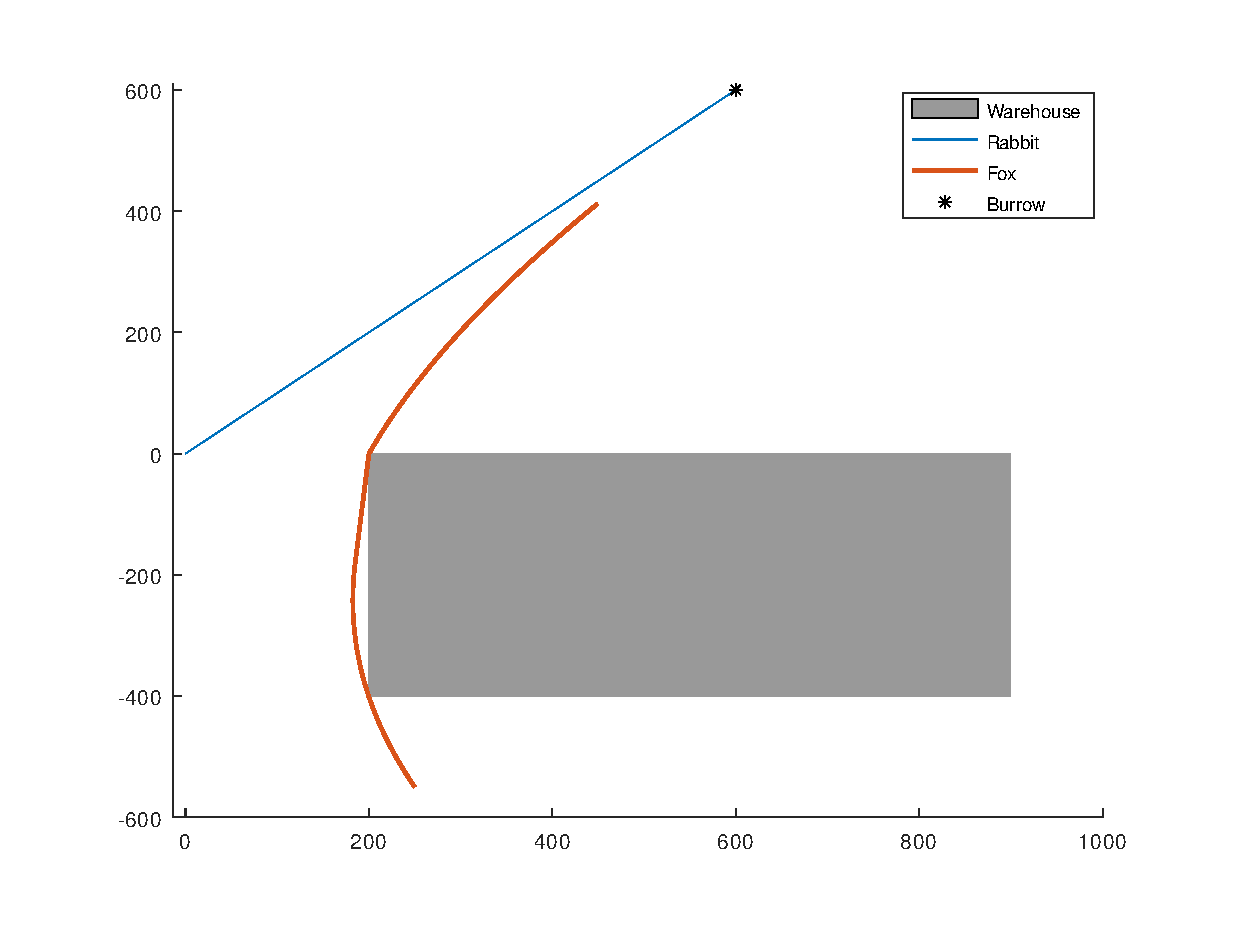
\includegraphics[scale=0.5]{simpleModel.eps}

      \label{fig:simplegraph}
\end{figure}
